\documentclass[a4paper,10pt]{article}
\usepackage{graphicx}
\usepackage[spanish]{babel}
\usepackage[latin1]{inputenc}
\usepackage{a4wide}
\usepackage{amsmath}
\usepackage{amssymb}
\usepackage{graphicx}
\usepackage{eqnarray}
\usepackage{epstopdf}
\usepackage{subfigure}
\usepackage{natbib}
\usepackage{algorithm}
\usepackage{hyperref}

\usepackage{amsfonts}  % For \mathbb
\usepackage{bm}   % command \bm

\usepackage{xcolor}
\usepackage{listings}
\lstset{basicstyle=\ttfamily,
  showstringspaces=false,
  commentstyle=\color{red},
  keywordstyle=\color{blue}
}

\begin{document}

\title{Crazyflie 2.1 - ROS (\texttt{uned\_crazyflie\_ros\_pkg})}
\author{Francisco J. Ma�as-�lvarez}     
\date{\today}
\maketitle
\tableofcontents
\newpage


\section{Introducci�n}
% -------------------------------------
\section{Visi�n general}
% -------------------------------------
\section{ROS}


\subsubsection{Crazyflie\_ros}
TO-DO
\begin{figure}[ht]
  \centering
    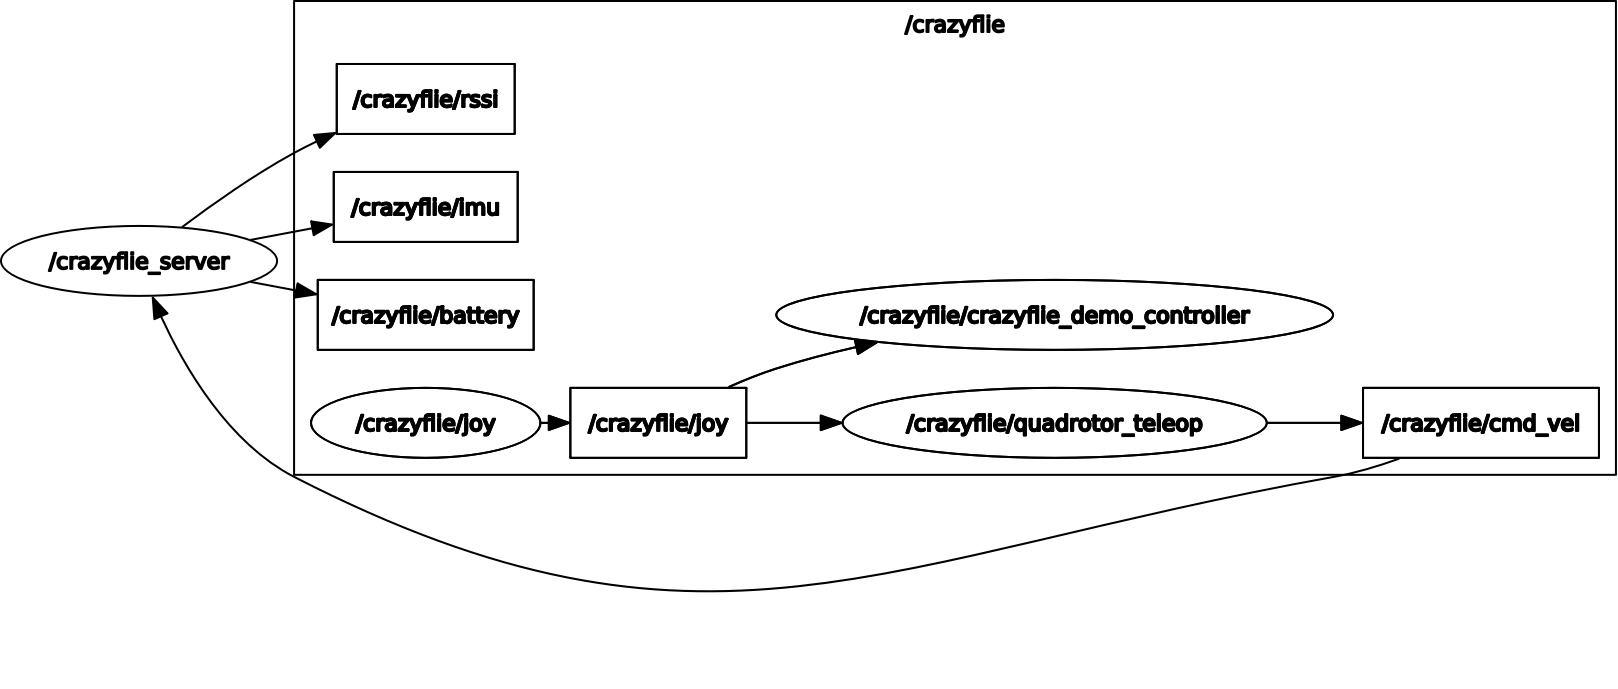
\includegraphics[width=1.0\textwidth]{figs/rosgraph.png}
  \caption{rosgraph.}
  \label{fig:rosgraph}
\end{figure}

%% ---------------------------------------------------------------
%%                         BIBLIOGRAPHY
%% ---------------------------------------------------------------
%\bibliographystyle{plain}
%\bibliography{refs}


\end{document}